\documentclass[letterpaper,12pt]{article}
\usepackage{graphicx}
\usepackage{subcaption}
\usepackage[english]{babel}
\usepackage{fancyhdr}
\usepackage{siunitx}

\graphicspath {{figures/}}

\setlength{\headheight}{15pt}

\pagestyle{fancy}
\fancyhf{}
\lhead{\textbf{Version:} 1.1  \textbf{Revision:} 11/02/17}
\rhead{\thepage}
\lfoot{Cole Kampa}
\rfoot{\textit{Mu2e: University of Minnesota}}

\renewcommand{\footrulewidth}{1pt}


\begin{document}
\begin{titlepage}
	\centering
	
\includegraphics[width=0.5\textwidth]{mu2e_logo_oval.png}\par\vspace{2cm}
	{\scshape\LARGE Standard Operating Procedure: Automated Straw Resistance Measurements\par}
	\vspace{3cm}
	{\Large Cole Kampa\par}
	\vspace{3cm}
	{\large University of Minnesota\par}
 	\vspace{.5cm}
	{\large November 2, 2017\par}
	% Bottom of the page
	\vfill
	{\verb|kampa041@umn.edu|\par}
\end{titlepage}

\clearpage
\setcounter{page}{2}


\section{Goal}
Immediately after removing the paper and before gluing in the CO$_{2}$ end pieces, the resistance of each straw will be measured and recorded. In an effort to diagnose any issues with the metalization in each straw, four resistances will be measured, all from the ends of the straws: inside-inside (i-i), inside-outside (i-o), outside-inside(o-o) (figure 1). Thus for each pallet 96 measurements must be taken. We strive to do this in a safe, efficient, and reproducible manner.

\begin{figure}[h]
	\centering
	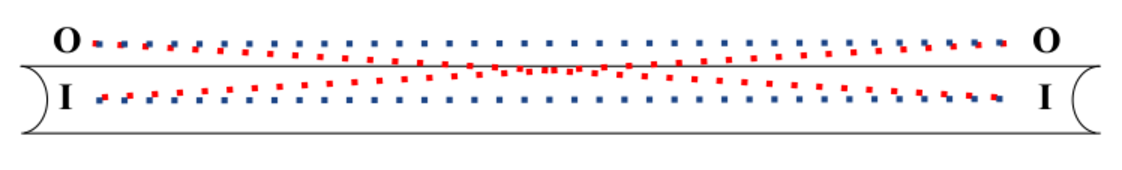
\includegraphics[width=\textwidth]{straw_meas_2}
	\caption{Diagram of different resistance measurements on each straw. Note that the cross measurements in red, inside-outside \& outside-inside, should have an infinite resistance.}
\end{figure}


\section{Equipment}
\begin{itemize}
	\item Full pallet of 24 Mylar straws (incremental numbering, st\#\#\#\#\# format)
	\item Resistance Meter v1.0 (Arduino Uno \& PCB in acrylic box) (figure 2)
	\item 9V power supply with barrel connector
	\item USB A to USB B cable
	\item Left and right resistance connectors and ribbon cables
	\item Aluminum bar covered in electrical tape
	\item Small, stainless steel scissors
	\item Computer with Python 3 and Mu2e-Factory repository cloned to Desktop (see readme.md for information on necessary Python libraries)
	\item Barcode scanner connected to computer via USB
	\begin{figure}[h]
		\centering
		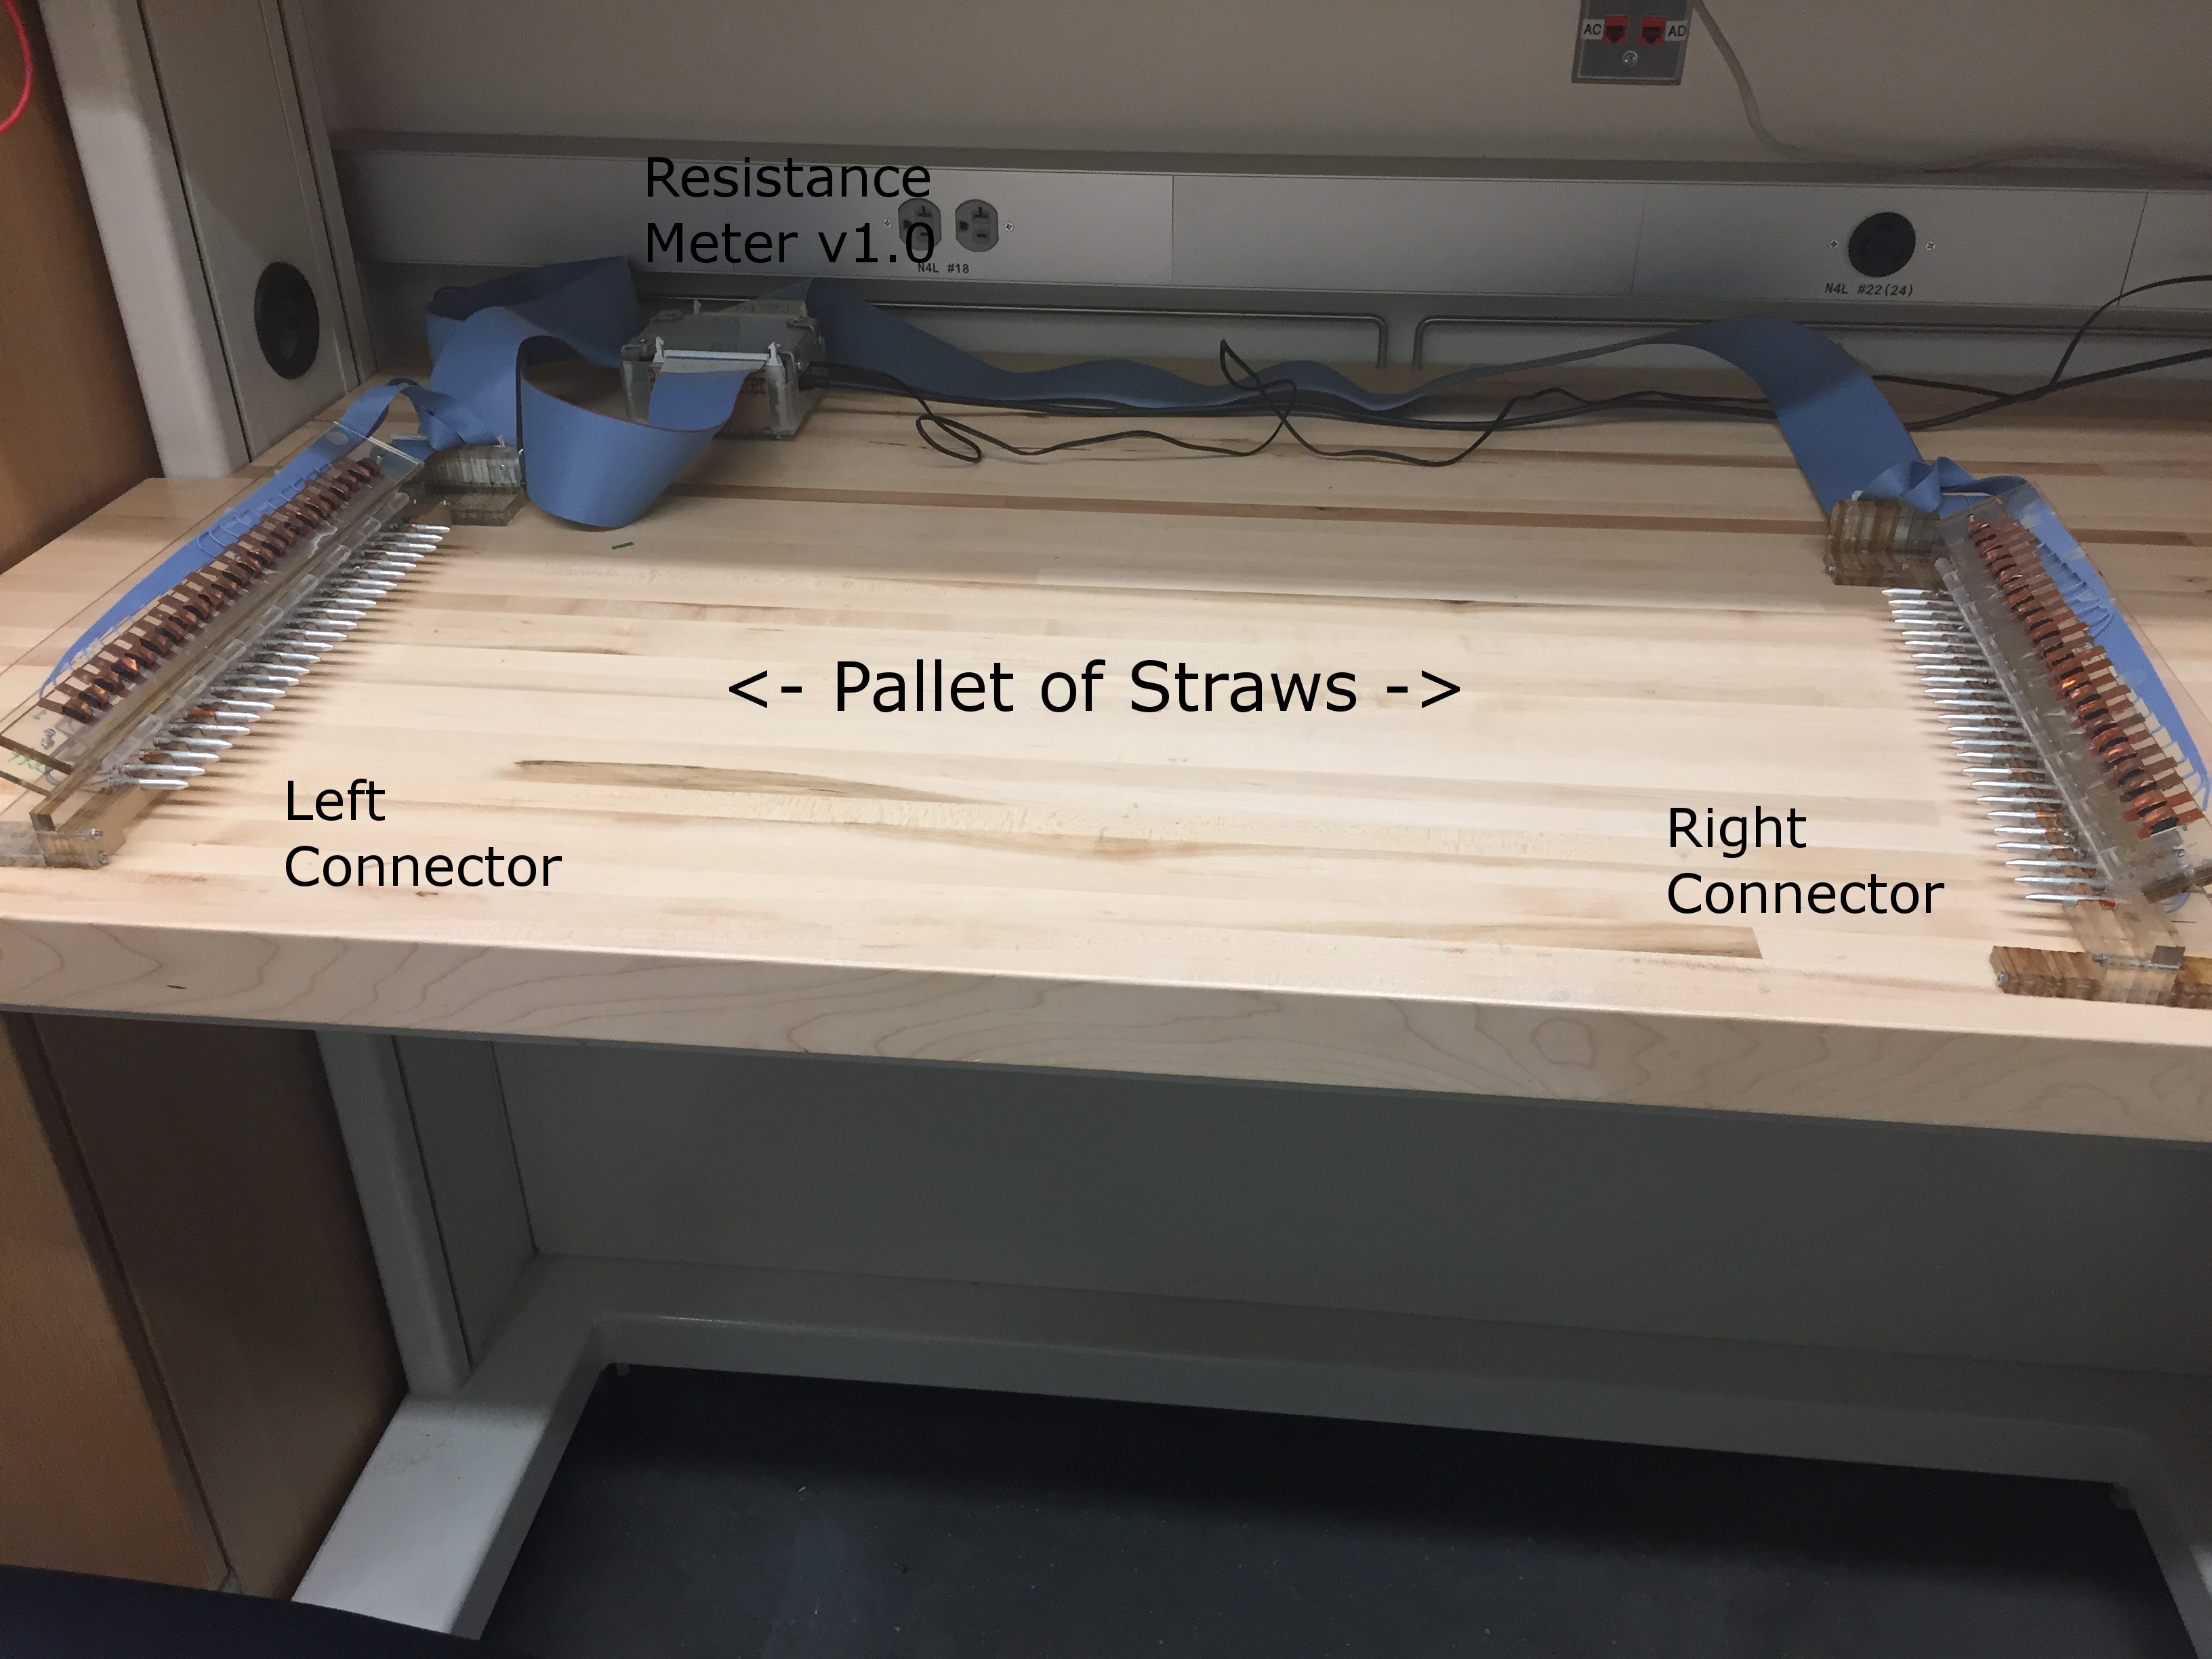
\includegraphics[width=\textwidth]{full_setup2_labeled}
		\caption{Full resistance meter setup labeled.}
	\end{figure}
\end{itemize}


\section{Important Files}
The following files are located in the Mu2e-Factory github repository (https://github.com/ckampa13/Mu2e-Factory), which is cloned to the computer used with this process on the desktop. All files are within the Mu2e-Factory/Resistance\_Measurement/Automated/ directory.

\begin{itemize}
	\item measurement.py (main script, measures straw resistance; shortcut located next to folder on desktop: Resistance Measurement)
	\item calib.csv (Directory: .../Calibration/ ; calibration data stored in this file)
	\item StrawResistance\_YYYY-MM-DD\_HHMMSS.csv (Directory: /Resistance\_Data/; measurement data stored using this naming convention)
\end{itemize}


\section{Risks and Dangers}
The primary risk associated with this measurement is the risk of damaging the straws. It is very important to follow the SOP carefully, otherwise straw kinks are likely to occur. Since the connector slides into the straws and pressure is on both the inside and outside metalization, there is also the possibility of scraping the straws. This should be avoided at all times.

\section{Resistance Measurement Procedure}
\subsection{Resistance Meter v1.0 Setup}
\begin{enumerate}
	\item Plug USB cable: USB B into “Resistance Meter v1.0” box Arduino Uno USB serial port and USB A into computer USB port (figure 3).
	\item Plug power supply (9V) into Arduino power port and outlet (figure 3).
	\item Plug connector labeled “Right” into matching ribbon cable. The other end of the ribbon cable should be plugged into the top of the Resistance Meter box ribbon cable connector labeled “Right”.
	\item Repeat (3) for “Left” connector. Note that the left cable has a given orientation to be plugged in and is labeled (“Left Box” and “Left Connector”).
\end{enumerate}

\begin{figure}[h]
	\centering
	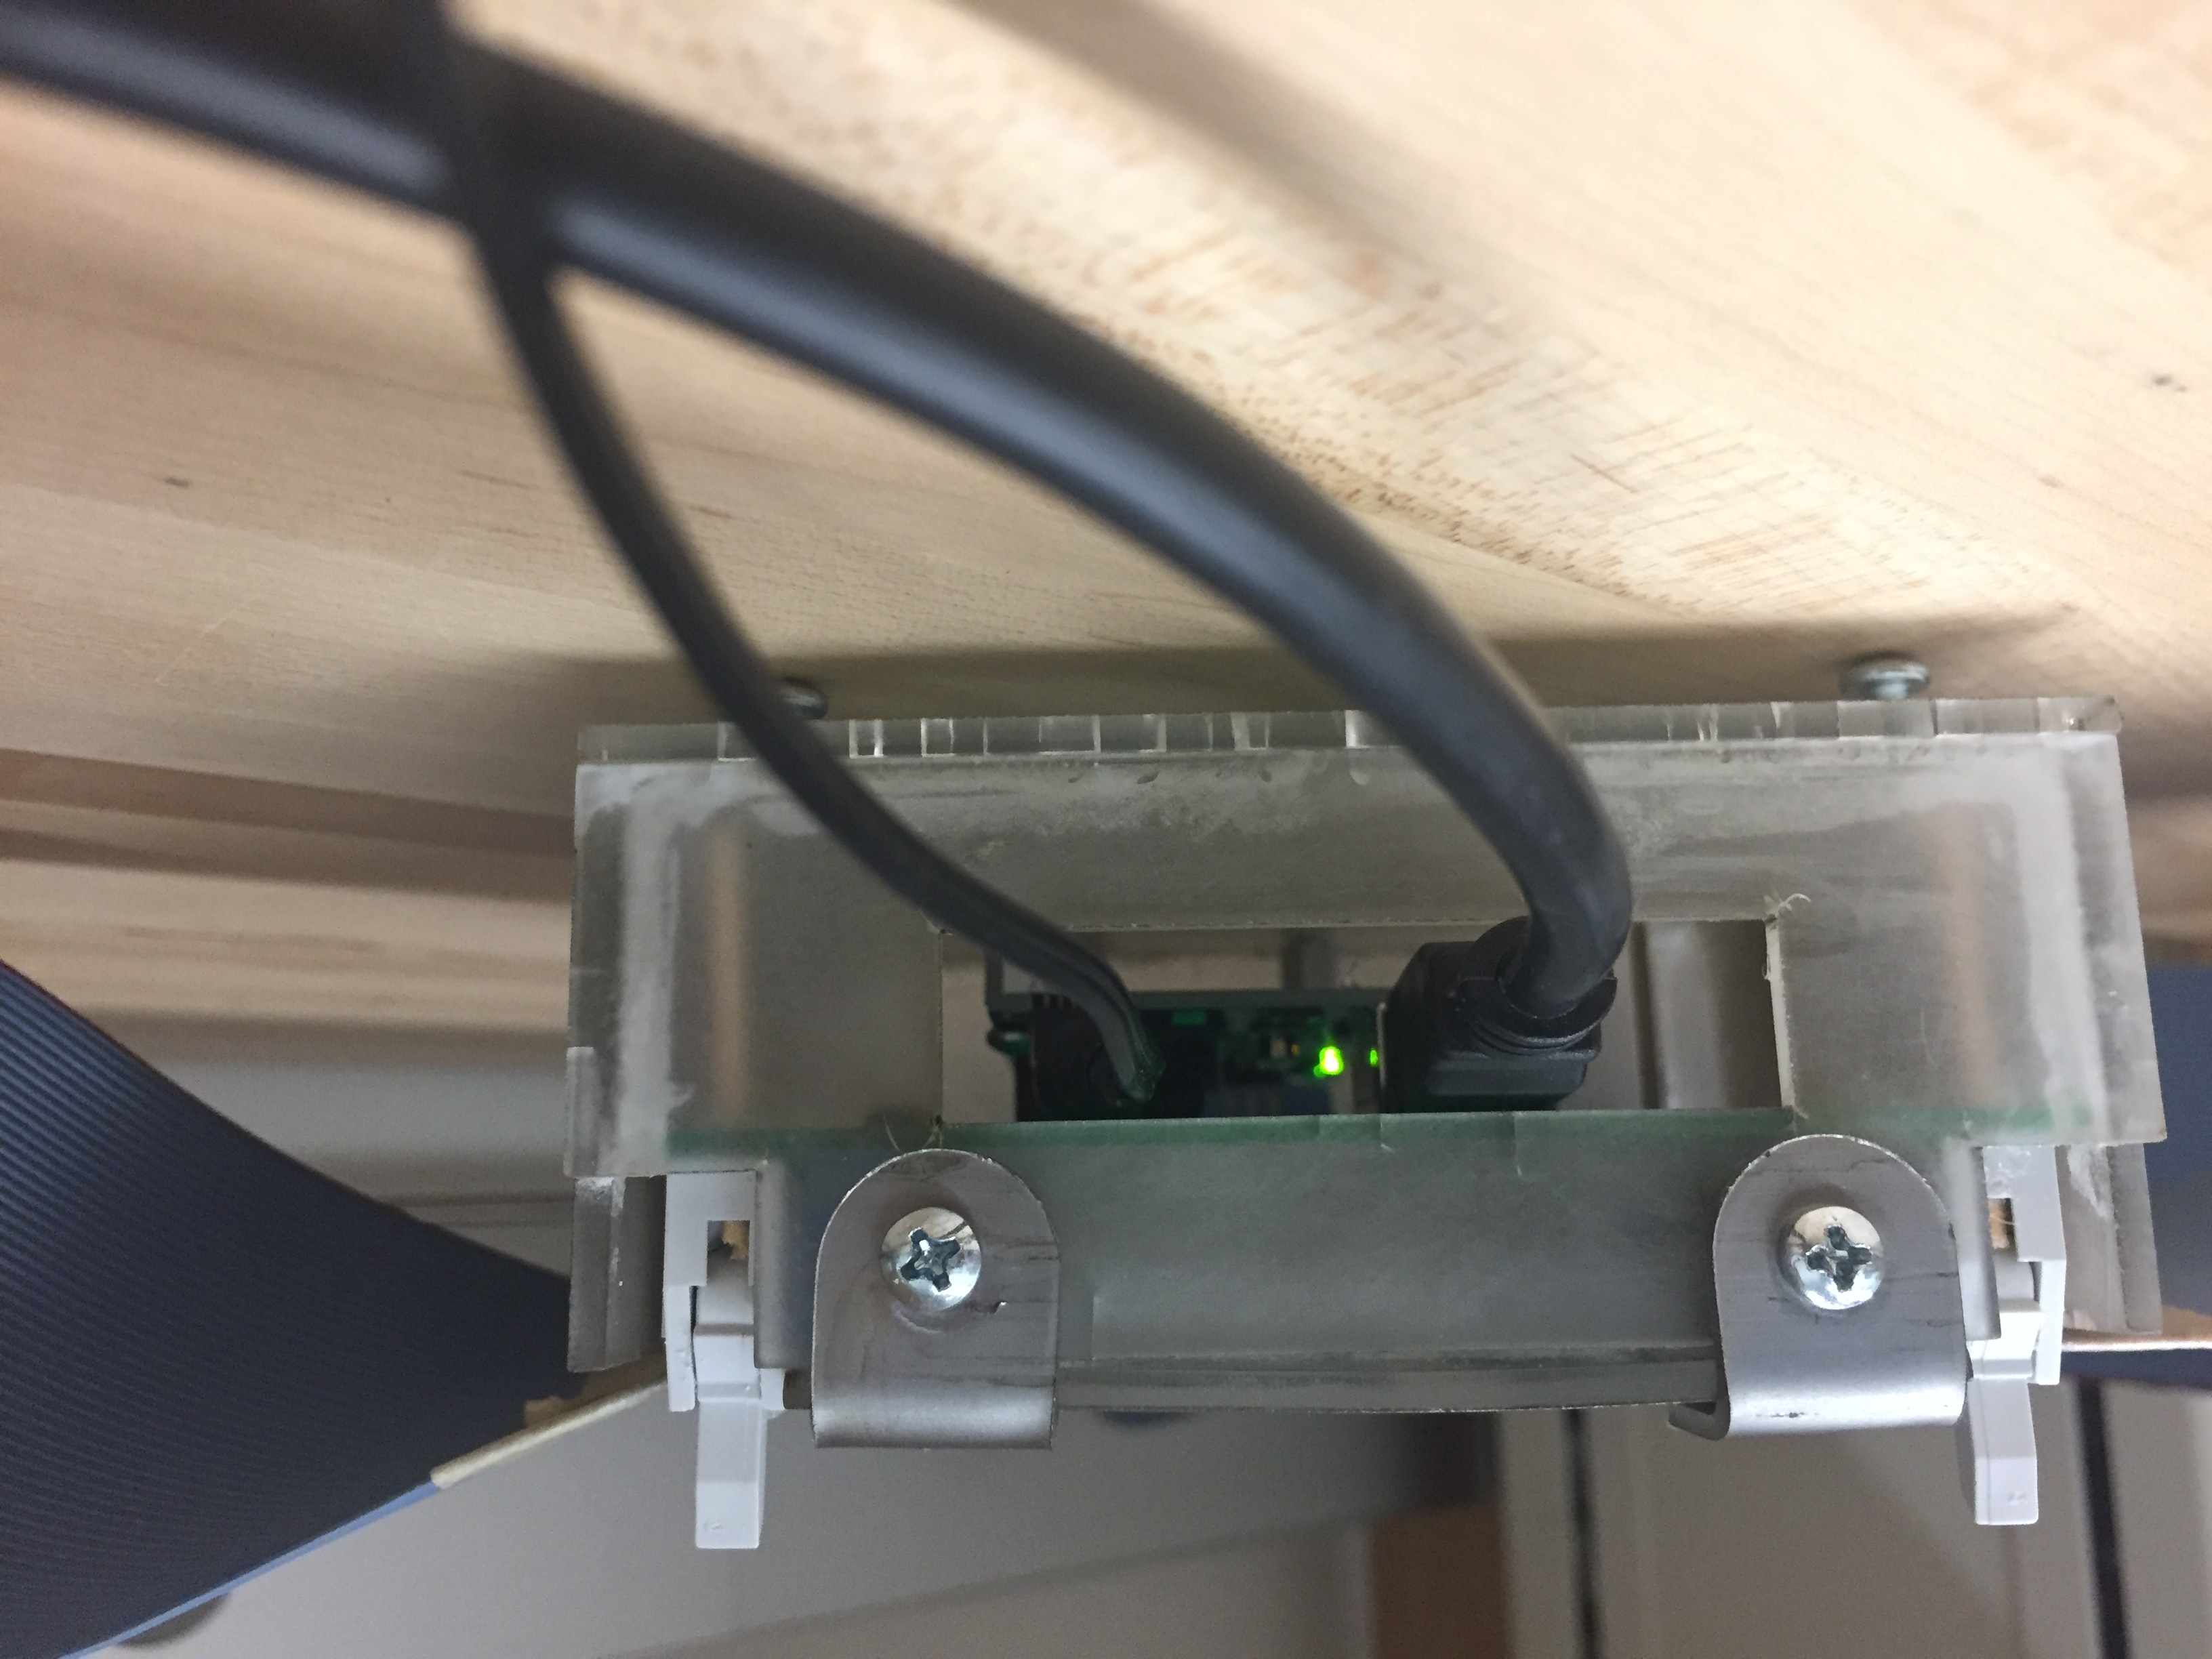
\includegraphics[width=\textwidth , angle=180]{resistance_box_plugged2}
	\caption{Plugged in Resistance Meter: USB cable on left, power supply cable on right.}
\end{figure}

\subsection{Connection to Straws}
\begin{enumerate}
	\item Put on nitrile gloves.
	\item Place pallet of straws on middle of desk.
	\item Using aluminum bar with electrical tape, gently push on the right ends of the straws (ie in direction to slide straws to the left in the pallet troughs) so that they are all aligned on the right side. This will likely cause the left side to be very uneven.
	\item Place right connector on far right side of pallet, with probes facing the straws. The connector should nest over the aluminum base of the pallet.
	\item Open top hinged half of the connector and slowly slide towards straws. As aluminum probes slide in the straws, it may be necessary to put light pressure on the center of the straws to prevent them from sliding. Slide probes all the way in.
	\item Using the scissors, cut the left end of the straws to as even a length as possible, while still allowing some of the straws to stick out of the troughs (this allows for better connections).
	\item Using the method described above, attach the left connector to the straws.
\end{enumerate}

\subsection{Collect Data}
\begin{enumerate}
	\item Open resistance test GUI from shortcut, named \verb|RUN_RESISTANCE_TEST|, on desktop. A screenshot of the GUI is shown in Figure \ref{gui}.
	\item Using barcode scanner at computer, scan worker ID and workstation ID
	\item Scan in the straw barcode for the lowest-numbered straw on the pallet into the box in the GUI.
	\item Have one person stand at the left connector. They should use their forearm to apply even pressure to the top of the left connector, while the operator applies even pressure to the right connector (figure 4).
	\begin{figure}[h]
		\centering
		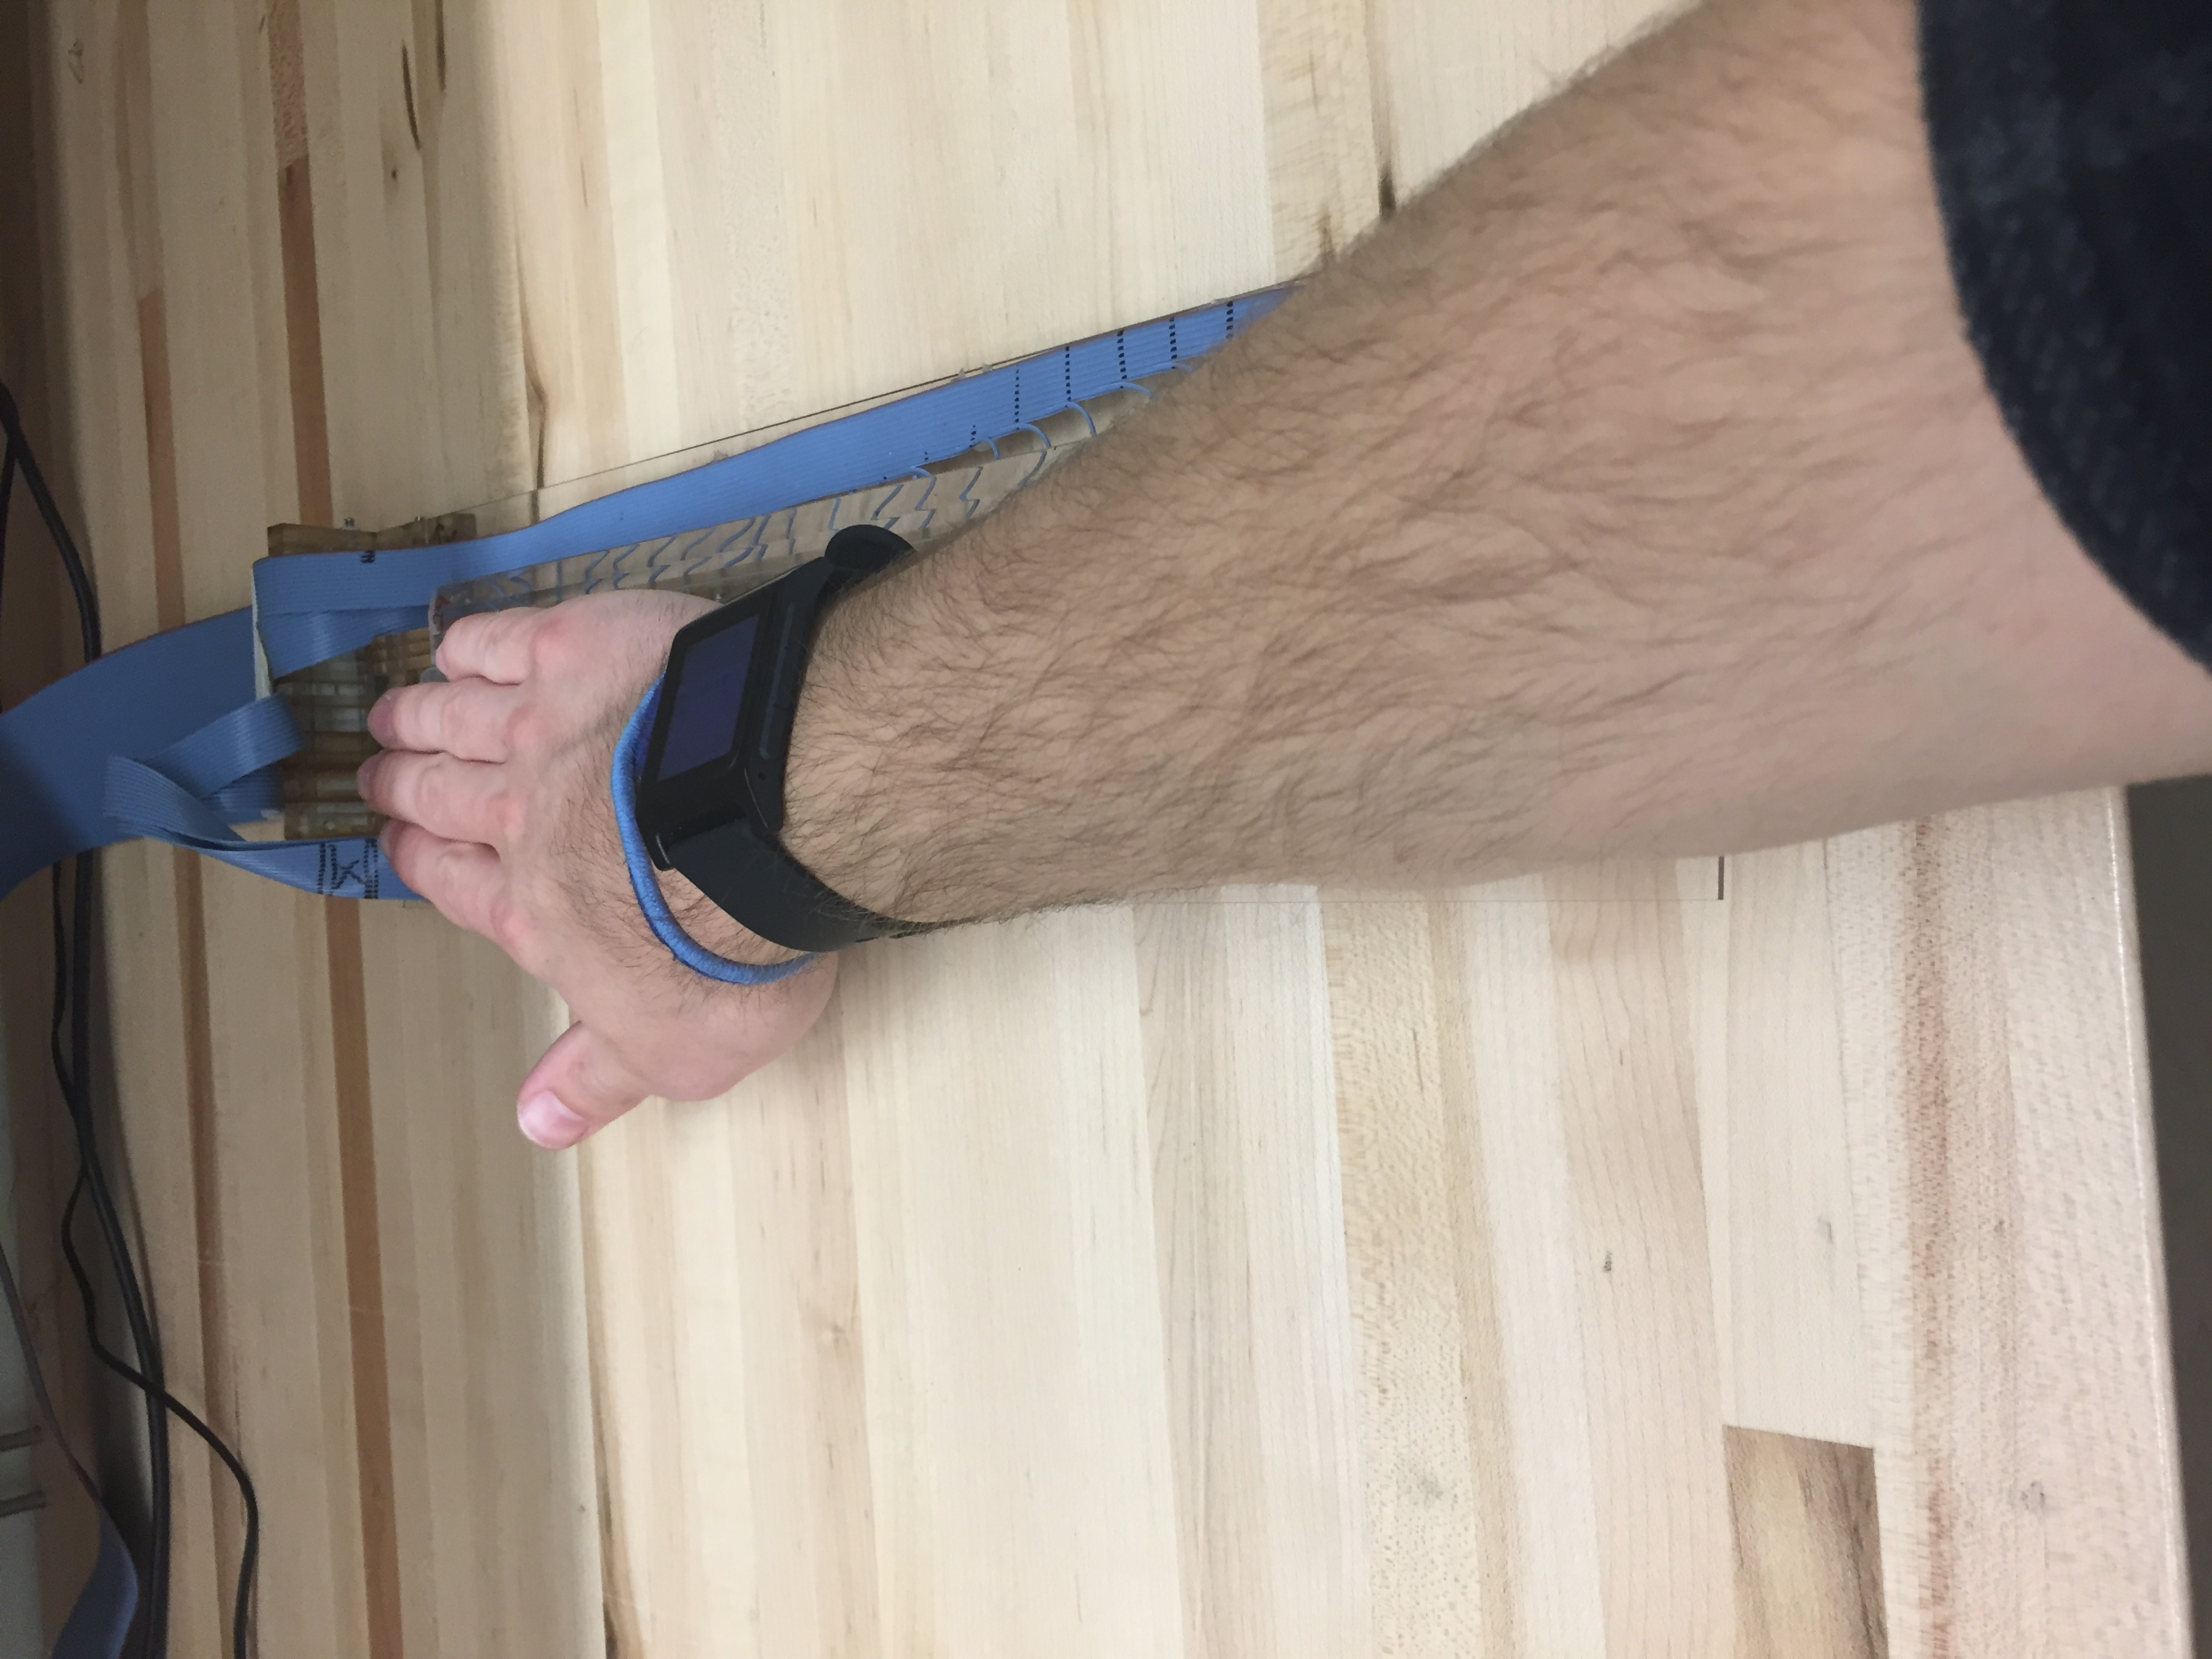
\includegraphics[scale=0.075 , angle=270]{closed_right_pressure}
		\caption{Putting pressure on the right connector. Make sure to wear gloves when connector is actually attached to straws.}
	\end{figure}
	\item Click on ``generate'' in the GUI to measure the resistances.
	\item The display will show measurements with pass or fail ratings, with green for pass and red for fail. To retest the straws that failed, simply hit ``generate'' again.
	\item The data saves automatically. When finished, either exit out of the program, or click on ``reset'' to test another pallet of straws.
\end{enumerate}

\begin{figure}
	\centering
	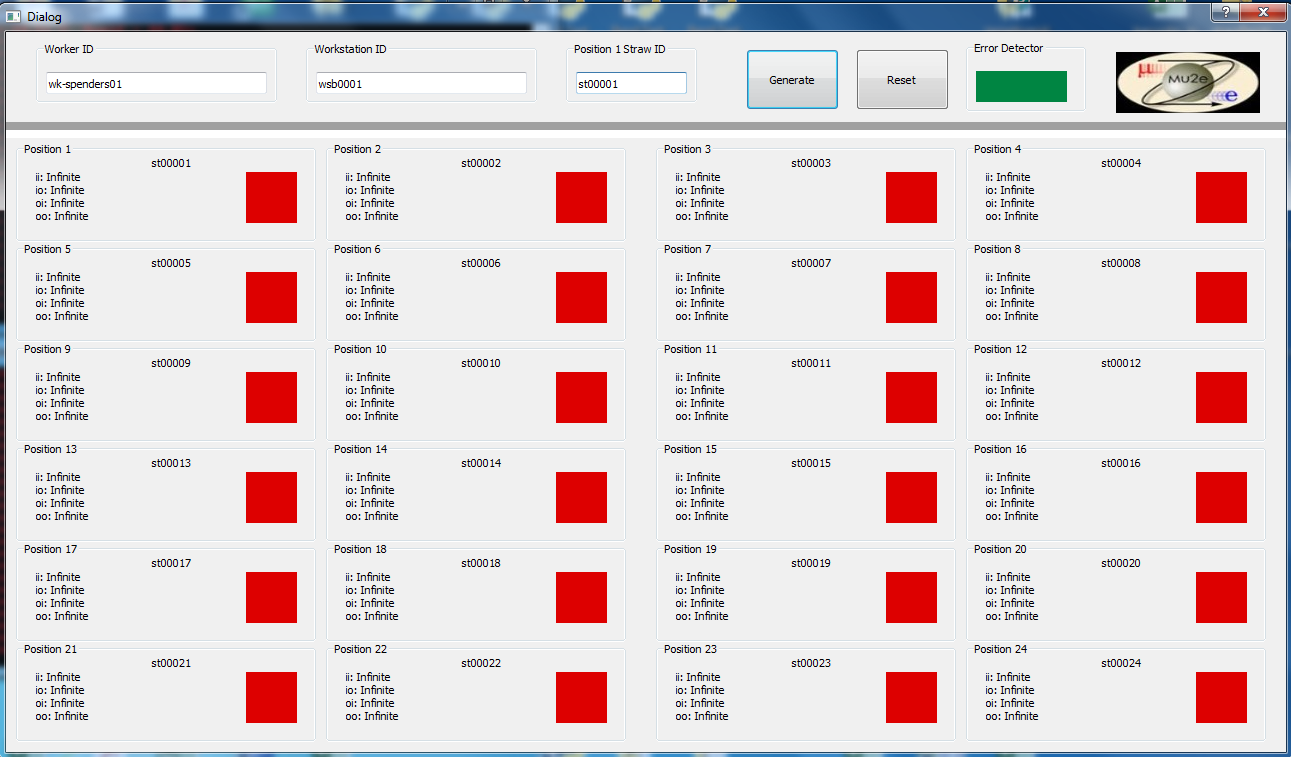
\includegraphics[width=\textwidth]{gui}
	\caption{Resistance testing GUI.}
	\label{gui}
\end{figure}

\subsection{Cleanup}
\begin{enumerate}
	\item Lift right connector top plate
	\item Slowly slide right connector out of straws, and store on back portion of desk
	\item Repeat for left connector
	\item Dispose of any small straw fragments from cutting process into trash bin
\end{enumerate}

\section{Troubleshooting}

If anything is unplugged, plug it in and try again (i.e. power, USB, ribbon cables on box end or connector end). If this does not work, immediately alert the workstation manager, who will replace entire setup with new resistance meter box and connectors (should have 2 sets at all times). When replacing, check serial port (using Arduino software) and adjust calib.py and measurement.py to reflect the change in port number. Then, run calib.py (see Calibration SOP), and proceed with production. \\

At a test computer, the manager/troubleshooter should plug malfunctioning box in to power and USB to the computer, and connect a 150$\Omega$ calibration pallet to the ribbon connectors on the box. Run the script to see if each channel reads approximately 150Ω. If they do, there is likely a bad connection somewhere within one or both of the connectors. 

Some other possible culprits are listed below.

\begin{enumerate}
	\item Script Crashes:
	\begin{itemize}
		\item First, run a command prompt (to prevent script from automatically closing) in the directory that the script is located (Shift+RClick on Windows 7 in File Explorer, select “Open Command Window Here”), then run the command 
$ \$ python measurement.py \$ $
		\item Take note of any errors that follow
	\end{itemize}
	\item Hardware Errors:
	\begin{itemize}
		\item Crashes immediately upon running:
		\begin{itemize}
		\item Verify Arduino is plugged in to power and USB to computer
		\item Using Arduino software, check port of board (‘COM\#\#’ on Windows, ‘dev/...’ on Linux) using Tools-Port (should be listed as Arduino Uno)
		\item make sure \verb|com_port| variable in \verb|measurement.py| line 42 matches port
		\end{itemize}
	\end{itemize}
	\item Typographical Errors:
	\begin{itemize}
		\item Fails at Temp or Humid:
		\begin{itemize}
		\item Make sure to enter int or float values
		\item Fails after entering start and end straws
		\item Verify format of ‘st\#\#\#\#\#’ where \# are digits 0-9
		\item Difference between start and end straw should be 23 (i.e. full pallet of 24 straws, in order)
		\end{itemize}
	\end{itemize}
	\item Bad Measurements:
	\begin{itemize}
		\item Check last time of calibration (kept in log sheet on desk above resistance meter)
		\item Try redoing calibration (see SOP for calibration)
		\item Make sure connections are solid
		\item One channel always reads zero ohms or inf when it shouldn’t:
		\begin{itemize}
		\item Use handheld multimeter to measure resistance from connection point at straw to cable end (see pinout diagrams). If resistance is high, check connection points along the way: ribbon connector (upside down), solder points (copper tape), copper tape to aluminum bullet in bottom half.
		\item Isolate problem and resolder if necessary
		\item Connect calibration pallet 1 (150 Ohm resistors) to resistance meter and run measurement.py, if channel still measures improperly, there might be a problem with the PCB (likely a failed multiplexer or a broken trace, which are not easy to fix. Put to side to be inspected by electronics specialist)
		\item Multiple lines going to the same analog input of Arduino (see pinout diagrams) are not working, test PCB with a new Arduino
		\item Test a new PCB if necessary
		\end{itemize}
	\end{itemize}
\end{enumerate}

%\section{Point of Contact}
%\begin{enumerate}
%	\item Project Head: Cole Kampa
%	\begin{itemize}
%		\item Email: kampa041@umn.edu
%		\item Phone: (715) 514-7796
%	\end{itemize}
%	\item Connector Design: Mitch Frand
%	\begin{itemize}
%		\item Email: frand053@umn.edu
%	\end{itemize}
%	\item Mu2e UMN: Dan Ambrose
%	\begin{itemize}
%		\item Email: ambr0028@umn.edu
%	\end{itemize}
%\end{enumerate}


\end{document}